\chapter{Characterization}
\graphicspath{{../gfx/chapter03/}{../plots/chapter03/}}


\section{The three-cell wire}

%
\begin{figure}
  \center
  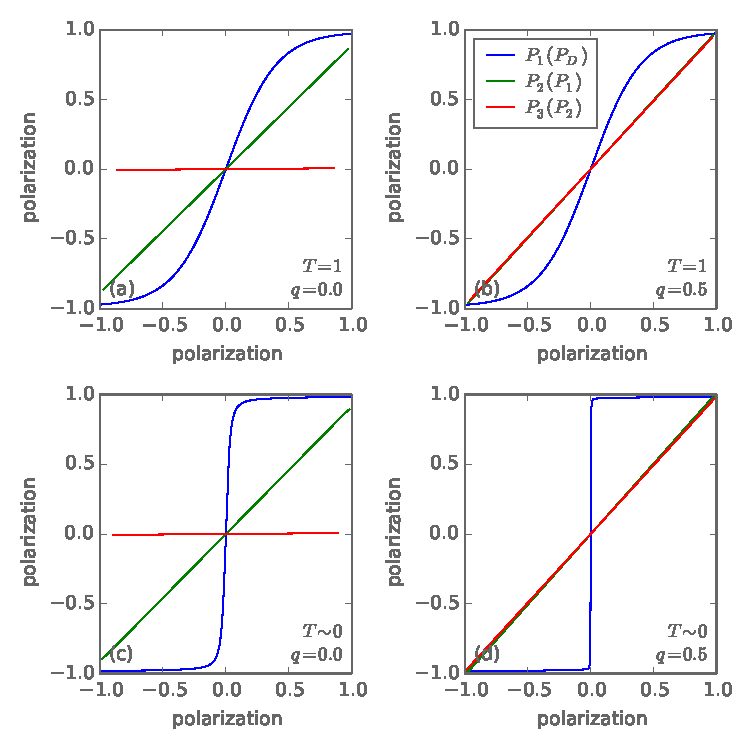
\includegraphics{three_cells_PP}
  \caption{
  }
  \label{fig:three_cells_PP}
\end{figure}
%
We choose a simple QCA system, the three-cell wire that we had already
introduced in Fig.~\ref{fig:short_wire}(b) in the first chapter, to investigate
general time-independent characteristics of QCA circuits. Specifically, we are
interested in how the polarization of one cell \emph{responds} to the
polarization of a second cell, and how cell polarizations depend on cell-cell
distance and inter-cell angle. For the nearest-neighbour Coulomb repulsion we
use $V_1 = 40$ and the cell-cell distance is $d/a = 2.2$, where $a$ is the edge
length of the cell. Most of our calculations will be at finite temperature, $T =
1$ and we will concentrate on horizontal wires for now (meaning the inter-cell
angle is $\theta = 0^{\circ}$). Both the Coulomb energy scale $V_1$ and the
temperature are in units of the hopping $t$, with $t = 1$.  For these parameters
the bond approximation is valid, which we deploy unless otherwise noted. We
investigate systems both without compensation charges $q = 0$, here the net cell
charge is $- 2 e$, and with a compensation charge of $q=\frac{1}{2}$, yielding
charge-neutral cells.

% ---

The driver cell sets the input for the three-cell wire with $P_D$ taking values
in the range $-1 \ldots 1$. The three active cells respond to the input
polarization. Formally, we can define the polarization response of cell $k$ with
respect to cell $l$ as

\begin{equation}
  \label{eq:polarization_response}
  \chi_{kl} = \frac{\partial P_k}{\partial P_l}\big|_{P_l = 0} \, .
\end{equation}

Fig.~\ref{fig:three_cells_PP}(a)~and~(b) show the polarization of the first cell
with respect to the driver cell, the polarization of the second cell with
respect to the first cell, and so on. For the first cell, the response is
non-linear and shows gain, therefore $\chi_{1D} > 1$. In contrast, the
polarization response between cells interior to the wire is linear and does not
exhibit gain, i.e.\ $\chi_{21} \le 1$ and $\chi_{32} \le 1$. Generally, the
polarization decreases monotonically from cell to cell, $|P_D| \ge |P_1| \ge
|P_2| \ge |P_3|$. In fact, for the $q=0$ system the polarization rapidly drops
to zero for the chosen parameters. The transmission is much improved for charge
neutral cells.  In that case, the response is almost perfect, $\chi_{21} \sim
\chi_{32} \sim 1$.

It is worth pointing out that at zero temperature, where we have to use the
fixed-charge model rather than the inapplicable bond approximation, we observe
the same polarization response characteristics. Quantitatively, for the same
system parameters the response is much improved at zero temperature compared to
$T=1$. But it remains true that the response inside the wire ($\chi_{21},
\chi_{32}$) is always linear and without gain.

In the literature, the non-linear nature of $P_1(P_D)$ has been noted
\cite{lent1993quantum} \cite{lent1993lines}, and the apparent gain $\chi_{1D} >
1$ has been invoked to argue for the robustness and fault-tolerance of the QCA
scheme. However, as our graph shows, this is only strictly true for the response
with respect to the driver cell. We believe that the picture where each cell
switches with gain with respect to its neighbours is an artifact of the ICHA
approximation, which treats each cell individually in the static charge mean
field of the other cells in the system. In other words, in the ICHA scheme, for
each cell the rest of the system is approximated by an effective driver cell.

%
\begin{figure}
  \center
  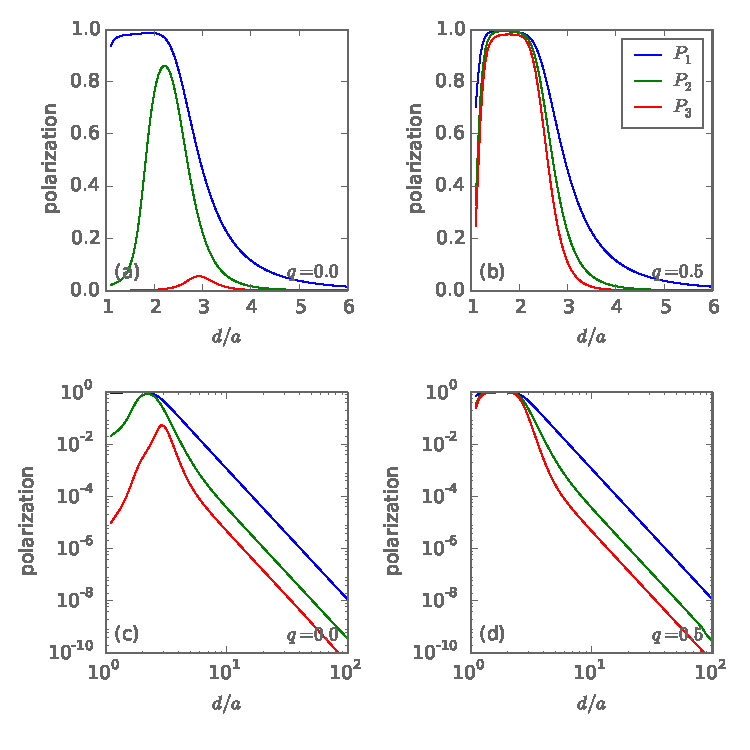
\includegraphics{three_cells_P_over_d}
  \caption{
  }
  \label{fig:three_cells_P_over_d}
\end{figure}
%

We now fix the driver polarization at $P_D = 1$ and look at how the
polarizations of the active cells depend on the cell-cell distance $d$, which we
report in units of the cell size $a$, see
Fig.~\ref{fig:three_cells_P_over_d}(a)~and~(b). At $d/a = 2$ all quantum dots in
the system are equally spaced, cells are placed a distance $a$ apart. At this
separation and smaller, our basic assumption of no inter-cell hopping breaks
down, as some dots in adjacent cells are now placed closer together than the
dots inside each cell. Thus $d/a \le 2$ is an unphysical limit. Conversely, at
very large cell-cell distances we expect the cells to become decoupled and
therefore all polarizations to be zero. Obviously, neither extreme limit is of
interest if our aim is to build functional QCA devices.

As already observed above, and in line with our intuition, polarizations
generally decrease from cell to cell as we go further away from the driver cell.
Without compensation charges ($q=0$) the polarization quickly falls off to very
small values, whereas for charge neutral cells ($q = \frac{1}{2}$) the situation
is much improved. (As far as we know, no one else has previously identified the
crucial role played by charge neutrality.)(Correction by Kevin.) The graph shows
that there is a cell-cell distance that yields maximal polarization for each
cell. For the $q=0$ system---non-charge-neutral cells---the optimal distance
increases from cell to cell, due to charge buildup. In contrast, with
charge-neutral cells ($q=\frac{1}{2}$) the cell-cell distance yielding optimal
polarization does not change notably from cell to cell. In fact, here a range of
distances gives very good polarizations, as the polarization saturates at values
close to $P = 1$. Of course, for a wire what really matters is the output
polarization. For the chosen parameters, this calculation demonstrates that for
a $q=0$ system we should choose $d/a \sim 3$. For $q=\frac{1}{2}$ the range $d/a
\sim 1.3 \ldots 2.3$ {[}more exact values!{]} gives the best output
polarization. Worryingly, this range is very close to the lower, unphysical
limit!

Especially for the non-charge-neutral system it is beneficial to allow for
different distances between different adjacent cells along the wire.  Thus a
single $d/a$ parameter is replaced by $d_k/a$ with $k = 1,2,3$ for the
three-cell wire. Using a stochastic optimization scheme we can optimize the
$d_k/a$ for optimal output polarization {[}reference{]}. We find that the output
polarization is significantly improved from $P_3 = 0.06$ for uniformly spaced
cells to $P_3 = 0.15$ for cells with individual cell-cell distances. Not
surprisingly, cells are farther spaced to the right (the output) and closer
spaced to the left (the input). This is a manifestation of charge buildup in the
system. The situation is very similar for longer wires and different parameters
for non-charge-neutral wires. We can do the same stochastic optimization for
charge-neutral wires ($q=1/2$), but find that little is gained by allowing
non-uniform cell-cell distances. Looking at Fig.~\ref{fig:three_cells_P_over_d}
this is really not surprising at all and in turn a consequence of having no
charge buildup in the system. It should be emphasized how much better the output
polarization is for charge-neutral wires. At least for the chosen parameters,
even very short wires seem unrealistic for a non-charge-neutral system.
% TODO: Kevin: Doesn't this have implications for the directionality of
% polarization signal transport?
% --- Yes, I should mention that. We should say that this demonstrates that in
% principle for a non-charge-neutral device we can optimize the functionality /
% output polarization by slightly moving cells around.

It is instructive to plot the polarizations over cell-cell distance up to very
large distances in a log-log graph as shown in
Fig.~\ref{fig:three_cells_P_over_d}(c)~and~(d). Even though large distances come
with extremely small polarizations that are not of practical interest, this
graph yields valuable insights into the nature of the interaction that mediates
the polarization. At distances $d/a > 10$ we see that the polarization settles
into an universal long range tail with $P(d) \sim d^{-5}$.  This is consistent
with our understanding that the polarization is mediated by a
quadrupole-quadrupole interaction. But remarkably, for these large distances the
polarization is exactly the same for both the $q=0$ and the $q=\frac{1}{2}$
systems. Hence, having non-charge-neutral cells does not actually alter the
characteristics of the cell-cell interaction. Instead, it suppresses the
cell-cell interaction at small distances. That is, charge repulsion competes
with the quadrupole interaction. Of course, we are mostly interested in small
distances, where the polarization is relatively large. This is the regime where
it is not quadrupolic and is suppressed for $q = 0$. For small distances the
polarization falls of faster than $d^{-5}$, thinking in terms of a multipole
expansion, we need to include higher-order corrections.

%
\begin{figure}
  \center
  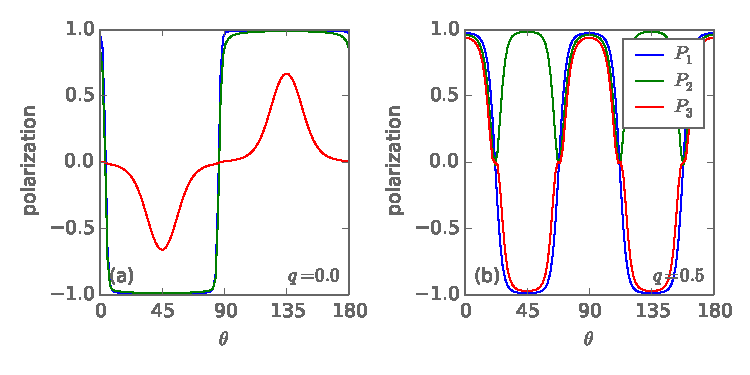
\includegraphics{three_cells_P_over_theta}
  \caption{
  }
  \label{fig:three_cells_P_over_theta}
\end{figure}
%
We expect the inter-cell angle to influence the polarization of the wire.
Therefore we explore the behaviour as we rotate the wire from a horizontal
configuration ($\theta = 0^{\circ}$) over a ``diagonal'' configuration ($\theta
= 45^{\circ}$) to vertical ($\theta = 90^{\circ}$) back to horizontal ($\theta =
180^{\circ}$) and look at the cell polarizations, shown in
Fig.~\ref{fig:three_cells_P_over_theta}. Alternatively, we can think of the
process as rotating the cells themselves about their centre while keeping the
wire unchanged. Let us start by looking at the charge-neutral system, with
$q=\frac{1}{2}$. The wire seems to work properly, i.e.~transmit a signal
reasonably well, within the angle ranges $\theta = n \cdot 45^{\circ} \pm
10^{\circ}$ where $n$ is an integer and the range depends on the specifically
chosen system parameters. In between those ranges are nodes, e.g.~at $\theta =
22.5^{\circ}$, which would obviously not be useful angles if we are trying to
transmit a signal, but might, in contrast, be very helpful if we are trying to
isolate cells from each other. An important detail is that for diagonal wires,
at $\theta = 45^{\circ}$, for example, the polarizations are alternating: $P_D
\sim 1, P_1 \sim -1, P_2 \sim 1,$ and $P_3 \sim -1$.  Considering the Coulombic
interactions in such a system, Fig.~\ref{fig:short_wire}(b), we convince us that
this is indeed the expected behaviour. We note that the system is invariant
under rotations by $90^{\circ}$.

The situation is very different for non-charge-neutral system, with $q=0$.
First, the system is rotationally invariant under $180^{\circ}$ which already
seems odd. Second, the graph shows that the magnitudes of the cell polarizations
are actually larger at $\theta \ne 0$ compared to $\theta = 0$. This is
especially impressive for $P_3$, with $|P_3| \sim 0$ at $\theta=0^{\circ}$ and
$|P_3| \sim 0.6$ at $\theta = 90^{\circ}$ {[}better numbers!{]}. But it is at
$\theta = 0$, the horizontal wire, where we know the systems behaves as
expected.  Therefore, we suspect that the cell polarizations are predominantly
set by the angle, and not by the driver polarization. Indeed, the same graph for
a driver polarization of $P_D = -1$ instead of $P_D = 1$ looks almost identical,
except for very small ranges of angles $\theta = n \cdot 90^{\circ} \pm
2^{\circ}$. This observation has far reaching consequences: The
non-charge-neutral system will never work as a QCA circuit unless all we want to
do is build linear chains of cells.  Even in this case the system becomes very
fragile with respect to angular displacement. Thus, for QCA charge-neutral
cells, $q=\frac{1}{2}$, are essential.


\section{Workable parameters for QCA}

%
\begin{figure}
  \center
  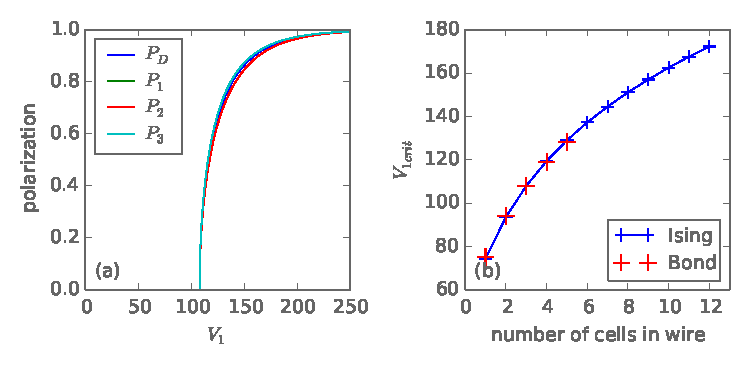
\includegraphics{critical_V1}
  \caption{
  }
  \label{fig:critical_V1}
\end{figure}
%

%
\begin{figure}
  \center
  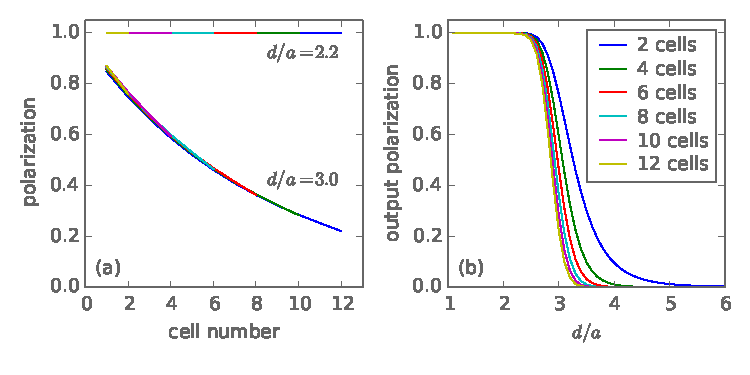
\includegraphics{wire_polarization}
  \caption{
  }
  \label{fig:wire_polarization}
\end{figure}
%
